\section{Quasiparticle excitations}
\label{sec:theory.quasiparticle}

\subsection{The quasiparticle density of states}
\label{sec:theory.quasiparticle.dos}

The quasiparticle excitations that are orthogonal to the ground state are neither lone electron nor hole excitations, but are superpositions of excitations on both sides of the Fermi surface.
These excitations are commonly called Bogoliubov quasiparticles, and I refer to them simply as quasiparticles.
They have spin $1 / 2$ and thus obey Fermi statistics.
Their canonical decay mechanism is to rejoin the condensate by recombining in pairs to form a Cooper pair and emitting a phonon.
Other decay channels are discussed below.

Because of the gap, there are no low-energy states into which the constituents of the Cooper pairs can individually scatter, and a supercurrent can thus flow with no resistance, at least at zero frequency.
However, like the conduction electrons of the normal metal, the quasiparticles experience lossy scattering.
Thus, the conductivity at nonzero frequencies, while typically much higher than in even an excellent normal conductor, is finite.
A KID detects radiation essentially by measuring these excitations through their effect on the surface impedance of the superconductor at microwave frequencies.

\todo[inline]{update after reading AM}
The energy of a Bloch state with wavevector $\vwvec$ is
$\blochenergy_{\vwvec} = \hbar^2 \wvec^2 / 2 \mass$
for an electron mass $\mass$.
If $\blochenergyf_{\vwvec} = \blochenergy_{\vwvec} - \blochenergy_\fermi$ is the same energy relative to the Fermi energy $\blochenergy_\fermi$, then the energy of a quasiparticle with wavevector $\vwvec$ is
\begin{equation}
\energy_{\vwvec}
  =
  \left( \blochenergyf_{\vwvec}^2 + \gap^2 \right)^{1/2},
\label{eqn:qpenergy}
\end{equation}
which is positive for excitations on both the ``electron'' branch outside the Fermi surface, with $\blochenergyf > 0$, and the ``hole'' branch inside the Fermi surface, with $\blochenergyf < 0$.
This relationship between the Bloch state energy and the quasiparticle energy is plotted in Figure~\ref{fig:quasiparticle_energy_and_density_of_states}(a).

\todo[inline]{Recreate BCS figure.}
\begin{figure}[htb]
\centering
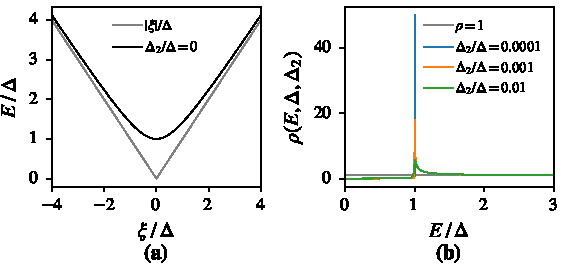
\includegraphics[width=\textwidth]{theory/quasiparticle_energy_and_density_of_states.pdf}
\caption
[The quasiparticle energy and density of states.]
{
\textbf{(a)}
The BCS quasiparticle energy $\energy$ versus the Bloch state energy $\blochenergyf$ in units of the gap.
Here, the Fermi energy is at $\blochenergyf = 0$.
\textbf{(b)}
The reduced density of states $\qprdos$ versus the quasiparticle energy $\energy$ in units of the gap.
For display, the three density of states curves have all been broadened by adding small imaginary parts to the gap:
$\gap \rightarrow \gap - \I \mitrovic$.
The gray horizontal line shows $\qprdos = 1$, which is the asymptotic value at high $\energy$.
%(If the corresponding energies were plotted in (a), they would have very narrow dips near $\blochenergyf = 0$ down to a minimum near $\energy / \gap = 0$.)
}
\label{fig:quasiparticle_energy_and_density_of_states}
\end{figure}

The range of energies involved forming the superconducting state is small compared to the Fermi energy.
Because the normal metal density of states does not change much over this range of energies, it is conventional to take it to be constant and to define $\ssdos$ to be the number of electron states of one spin per unit energy per unit volume at the Fermi energy.
The BCS density of states arises from the relationship between the quasiparticle energy $\energy$ and the Bloch energy $\blochenergyf$:
\begin{equation}
\dd{\energy}
  =
  \dd{\left( \blochenergyf^2 + \gap^2 \right)^{1/2}}
  =
  \frac{\blochenergyf \dd{\blochenergyf}}{\left( \blochenergyf^2 + \gap^2 \right)^{1/2}},
\end{equation}
so
\begin{equation}
\dd{\blochenergyf}
  =
  \frac{\energy \dd{\energy}}{\left(\energy^2 - \gap^2 \right)^{1/2}}.
\end{equation}
The density of quasiparticle states is thus
\begin{equation}
\supssdos(\energy)
  =
  \ssdos \dv{\blochenergyf}{\energy}
  =
  \ssdos \frac{\energy}{(\energy^2 - \gap^2)^{1/2}}
  \equiv
  \ssdos \qprdos(\energy),
\label{eqn:supssdos}
\end{equation}
where $\qprdos$ is the \textit{normalized} (or \textit{reduced}) density of states.
There is a one-to-one correspondence between the Bloch states and the quasiparticle states, so the total number of states is the same as for the normal metal.
The quasiparticle density of states versus quasiparticle energy is plotted in Figure~\ref{fig:quasiparticle_energy_and_density_of_states}(b).

While the BCS density of states has a singularity at $\energy = \gap$, in an actual superconductor this singularity will be smeared out at least slightly.
A supercurrent, always present in an operating KID due to the readout tone, causes some broadening of the density of states~\autocite{Anthore2003PRL}, as may granularity~\autocite{Dynes1984PRL}, disorder~\autocite{Driessen2012PRL}, and impurities~\autocite{ONeil2008PRL, ONeil2010JAP} in the film.
Such broadening of the density of states is often modeled, at least for energies near the gap, by writing the BCS reduced density of states as
\begin{equation}
\qprdos(\energy)
  =
  \Re{\frac{\energy}{(\energy^2 - \gap^2)^{1/2}}}
\end{equation}
and introducing a small imaginary part to either the quasiparticle energy
$\energy \rightarrow \energy - \I \dynes$~\autocite{Dynes1984PRL}
or the gap energy
$\gap \rightarrow \gap - \I \mitrovic$~\autocite{Mitrovic2008JPCM}.
Figure~\ref{fig:quasiparticle_energy_and_density_of_states}(b) shows density-of-states curves calculated using the latter procedure.
Both of these expressions describe a nonzero density of states for energies $\energy < \gap$.
The density of states may be measured in tunneling experiments, for example, but since we have not performed such experiments I will assume it changes little from the BCS form.
Although the density of states may be identically zero below some energy $\energy_\mathrm{min}$, with $\gap \ge \energy_\mathrm{min} > 0$, I will allow for the possibility of sub-gap states by writing integrals over quasiparticle energy with their lower limit set to 0, taking the cutoff to be present in the density of states.

In superconductor out of thermal equilibrium, the quasiparticle occupancy may differ between pairs of wavevectors on either side of the Fermi surface that correspond to quasiparticle states with the same energy, and may also differ between two spin states with the same wavevector.
Fortunately, we can ignore these distinctions.
The relevant quasiparticle excitation mechanisms, namely photons and phonons, populate both branches and both spin states equally on average~\autocite{Tinkham2004}.
In the absence of spin injection and external magnetic fields, we do not expect significant splitting of the density of states for opposite spin directions~\autocite{Meservey1970PRL}.
Thus, we can adequately describe the quasiparticle system using an occupancy function $\qpoccupancy(\energy)$ that has the same dependence on the quasiparticle energy for both branches and for both spin directions.
In thermal equilibrium at temperature $\temperature$, the occupancy is 
$\qpoccupancy(\energy, \temperature) = [\exp(\energy / \kb \temperature) + 1]^{-1}$,
the Fermi-Dirac function.
However, KIDs are typically operated out of equilibrium.

The quasiparticle density for an arbitrary $\qpoccupancy(\energy)$ is
\begin{equation}
\qpdensity
  =
  4 \ssdos
  \int_{0}^{\infty} \dd{\energy}
  \qprdos(\energy) \qpoccupancy(\energy),
\label{eqn:qpdensity}
\end{equation}
where one factor of two comes from the branches on either side of the Fermi energy, and the other comes from a sum over spins.
At low temperatures the gap will be close to its zero-temperature value $\gap_\zerotemp$, and the Fermi-Dirac occupancy is approximately
$\qpoccupancy(\energy) \approx \exp (-\energy / \kb \temperature)$.
Then, as derived in Appendix~\ref{chp:first-order_response}, the quasiparticle density is
\begin{equation}
\qpdensity(\temperature)
  =
  4 \ssdos \gap_\zerotemp
  K_1(\gap_\zerotemp / \kb \temperature)
  \approx
  4 \ssdos \gap_\zerotemp
  \left( \frac{\pi \kb \temperature}{2 \gap_\zerotemp} \right)^{1/2}
  \exp \left( -\frac{\gap_\zerotemp}{\kb \temperature} \right),
\label{eqn:qpdensity_thermal}
\end{equation}
where $K_1$ is the first-order modified Bessel function of the second kind.
These approximate expressions are plotted in Figure~\ref{fig:reduced_thermal_qpdensity}.
\todo[inline]{Recreate $\qpdensity$ figure and compare to exact BCS expression.}
The quantity $\ssdos \gap_\zerotemp$ frequently appears (usually with a prefactor of 2 or 4) as a characteristic quasiparticle density.
For aluminum,
$\ssdos \gap_\zerotemp \approx \SI{3.4e6}{\micro\meter^{-3}}$,
which is much larger than a typical operating density.
The quasiparticle density is discussed in more detail in Section~\ref{sec:theory.qpnumber}, where it replaces the occupancy as the quantity used to describe the quasiparticle system.

\begin{figure}[htb]
\centering
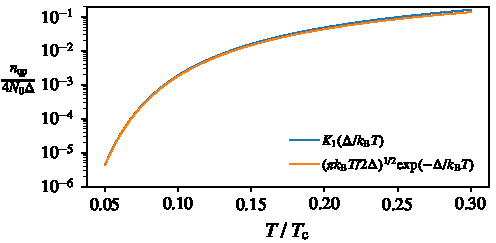
\includegraphics[width=\textwidth]{theory/reduced_thermal_qpdensity.pdf}
\caption
[The reduced thermal quasiparticle density versus reduced temperature.]
{The reduced thermal quasiparticle density versus reduced temperature, from Equation~\ref{eqn:qpdensity_thermal}.
The gap $\gap$ here is taken to be equal to its value at $\temperature = 0$, which at higher temperatures is not a good approximation.}
\label{fig:reduced_thermal_qpdensity}
\end{figure}

The quasiparticles affect the gap energy, which decreases as the quasiparticle density increases.
The BCS theory gives an implicit equation for the gap:
\begin{equation}
1
  =
  \ssdos \ucvolume \bcspotential
  \int_\gap^\infty \dd{\energy}
  \qprdos(\energy) \frac{1 - 2 \qpoccupancy(\energy)}{\energy},
\end{equation}
where the gap appears in both the lower limit of the integral and in the quasiparticle energy.
(The unit cell volume appears here because I use $\ssdos$ to mean the number of single-spin normal-metal states per unit energy \textit{per unit volume} at the Fermi energy.)
In Section~\ref{sec:theory.perturbation} I discuss a method for obtaining approximate equations for the gap.
Even in an illuminated KID, the number of excitations will generally be sufficiently small that the gap will not vary much from its value at zero temperature.


\subsection{Generation}
\label{sec:theory.quasiparticle.generation}

The quasiparticle excitations must occur in pairs, since the energy reduction is due to the pairing, so a particle that deposits energy greater than $2 \gap$ (the \textit{spectroscopic} gap) can break one or more Cooper pairs, exciting quasiparticles that eventually recombine into Cooper pairs or decay by other means.
Phonons with energy $\phononenergy > 2 \gap$ that enter the film from the substrate may also break pairs.

As we will see later, the detector sensitivity may be increased by using a high readout tone power.
Although the readout photons individually have energies much less than the gap (see Table~\ref{tab:energies}), a quasiparticle that absorbs many quanta and is excited to an energy above $3 \gap$ may scatter inelastically and create a phonon that is sufficiently energetic to break a pair.
KID experiments that use careful shielding to reduce quasiparticle generation due to stray light nevertheless observe more quasiparticles than the thermal equilibrium value, and some of this excess is typically attributed to readout generation~\autocite{deVisser2012APL,deVisser2014NatComm}.


\subsection{Pair recombination}
\label{sec:theory.quasiparticle.pair_recombination}

Quasiparticles have finite lifetimes and may decay in various ways.
For elemental BCS superconductors, the most relevant process involves two quasiparticles with energies
$\energy_1, \energy_2 \ge \gap$
recombining into a Cooper pair with the emission of a phonon with energy
$\phononenergy = \energy_1 + \energy_2 \ge 2 \gap$.
(Since a photon can break a Cooper pair and excite quasiparticles, the reverse process of recombination with photon emission is possible.
However, because the final density of states corresponding to this process is much smaller than the density of states for phonon emission, the radiative lifetime is much longer and this process is negligible~\cite{Burstein1961PRL}.)
\todo[inline]{Incorporate other refs in Rothwarf and Taylor}

\textcite{Kaplan1976PRB} derive a low-temperature equilibrium pair-recombination time, given for a quasiparticle with $\energy = \gap_\zerotemp$ by
\begin{equation}
\qprecombinationtime^{-1}
  =
  \electronphonontime^{-1}
  \pi^{1/2}
  \left( \frac{2 \gap_\zerotemp}{\kb \tc} \right)^{5/2}
  \left( \frac{\temperature}{\tc} \right)^{1/2}
  \exp \left( -\frac{\gap_\zerotemp}{\kb \temperature} \right),
\label{eqn:qprecombinationtime}
\end{equation}
where $\electronphonontime$ is the characteristic electron-phonon interaction time defined in the same reference.
The recombination rate for a given total energy is proportional to the phonon density of states at that energy, which increases with increasing energy~\autocite{Chang1978JLTP}.
Thus, quasiparticles with higher energies have shorter lifetimes.
Comparing Equation~\ref{eqn:qprecombinationtime} to Equation~\ref{eqn:qpdensity_thermal} shows that, in thermal equilibrium, the inverse recombination lifetime is proportional to the quasiparticle density:
\begin{equation}
\qprecombinationtime^{-1}
  =
  \electronphonontime^{-1}
  \left( \frac{2 \gap_\zerotemp}{\kb \tc} \right)^3
  \frac{\qpdensity}{4 \ssdos \gap_\zerotemp}.
\end{equation}
The proportionality
\begin{equation}
\qprecombination
  \equiv
  \left( \frac{2 \gap_\zerotemp}{\kb \tc} \right)^3
  \left( 4 \ssdos \gap_\zerotemp \electronphonontime \right)^{-1}
\label{eqn:qprecombination}
\end{equation}
is the quasiparticle recombination constant~\autocite{Gray1981Chapter5}.
Using values for aluminum from Table~\ref{tab:materials} gives
$\qprecombination = \SI{7.8}{\micro\meter^3.\second^{-1}}$.
The recombination constant will actually change as the gap energy varies with quasiparticle density~\autocite{Gray1971JPF, Rothwarf1974PRL}, but I will neglect this dependence.
The recombination rate per unit volume is thus quadratic in the quasiparticle density:
\begin{equation}
\rate_\qprecombination
  \equiv
  \qprecombinationtime^{-1} \qpdensity
  =
  \qprecombination \qpdensity^2.
\label{eqn:rate_qprecombination}
\end{equation}
Since recombination involves quasiparticles interacting in pairs, it is not surprising that the rate for $\qpnumber$ quasiparticles goes as $\binom{\qpnumber}{2} \propto \qpnumber^2$ to leading order~\autocite{Gray1971JPF}.

In thermal equilibrium, if quasiparticles are generated at a rate $\rate_\generation(\temperature)$ per unit volume and the only quasiparticle decay process is recombination with phonon emission, then the rate equation for the quasiparticle density is
\begin{equation}
0
  =
  \dv{\qpdensity}{\time}
  =
  \rate_{\generation}(\temperature)
  -
  \qprecombination \qpdensity(\temperature)^2.
\label{eqn:rate_qpdensity_thermal}
\end{equation}
Then, using Equation~\ref{eqn:qpdensity_thermal}, the low-temperature thermal generation rate is
\begin{equation}
\rate_{\generation}(\temperature)
  =
  \frac{4 \ssdos \gap_\zerotemp}{\electronphonontime} \left( \frac{2 \gap_\zerotemp}{\kb \tc} \right)^3 K_1(\gap_\zerotemp / \kb \temperature)^2
  \approx 
  \frac{4 \ssdos \gap_\zerotemp}{\electronphonontime} \left( \frac{2 \gap_\zerotemp}{\kb \tc} \right)^3 \frac{\pi \kb \temperature}{2 \gap_\zerotemp} \exp \left(-\frac{2 \gap_\zerotemp}{\kb \temperature}\right).
\label{eqn:rate_generation_thermal}
\end{equation}
At sufficiently low temperatures the total thermal generation rate will become negligible compared to other sources.
This reduces the effect of fluctuations in the generation rate cause by temperature fluctuations, which are common in a moving telescope.


\subsection{Phonons}
\label{sec:theory.quasiparticle.phonons}

While the various generation process act to create an occupancy that exceeds the thermal value, scattering processes act to restore the quasiparticle system to equilibrium.
\textcite{Kaplan1976PRB} derive a thermal equilibrium quasiparticle-phonon scattering time given by
\begin{equation}
\qpphononscatteringtime^{-1}
  =
  \electronphonontime^{-1} \Gamma \left(\tfrac{7}{2}\right) \zeta \left(\tfrac{7}{2}\right) \left( \frac{\kb \tc}{2 \gap_\zerotemp} \right)^{1/2} \left( \frac{\temperature}{\tc} \right)^{7/2},
\label{eqn:electron-phonon_scattering}
\end{equation}
where $\Gamma$ is the Gamma function and $\zeta$ is the Riemann zeta function.
Assuming the BCS weak-coupling relation, the numerical factors work out to
$\Gamma (7 / 2) \zeta (7 / 2) / 3.52^{1/2} \approx 1.996$.
\todo[inline]{Give scattering time with fiducial parameters.}
A quasiparticle at the gap edge cannot scatter and emit a phonon, because there no available quasiparticle states with lower energy, but at higher energies the scattering rate rapidly increases.
\todo[inline]{What about impurity scattering?}
\todo[inline]{What is the effect of electron-electron scattering? Allegedly important for aluminum. See ChangJLTP1978.}

A phonon produced by quasiparticle recombination has sufficient energy to break another Cooper pair in the same superconductor.
Such a phonon will quickly encounter the film-substrate interface, but the acoustic match between superconducting films and typical crystalline substrates tends to be poor, so phonons are likely to reflect on each encounter with the  interface~\autocite{Kaplan1979JLTP}.
These facts will significantly modify the results of the preceding section.

%In aluminum, \textcite{Kaplan1976PRB} calculate an average time $\phononpairbreakingtime = \SI{242}{ps}$ for a sufficiently energetic phonon to break a Cooper pair at low temperature, and the time decreases with increasing phonon energy.
\textcite{Chang1978JLTP} calculate a time
$\phononpairbreakingtime \sim \SI{100}{ps}$
for a sufficiently energetic phonon to break a pair, which is much less than both the inelastic scattering time and the anharmonic decay time~\autocite{Kozorezov2000PRB}.
They also calculate a phonon escape time
\begin{equation}
\phononescapetime
  =
  \frac{4 \thickness}{\efficiency \soundspeed},
\label{eqn:phononescapetime}
\end{equation}
where $\thickness$ is the film thickness, $\soundspeed$ is the speed of sound, and $\efficiency$ is the transmission probability per encounter, which may be quite small~\autocite{Kaplan1979JLTP}.
Using
$\thickness = \SI{40}{nm}$
and
$\soundspeed = \SI{6.4e3}{m.s^{-1}}$~\autocite{Chang1978JLTP}
gives
$\phononescapetime = \SI{25}{ps} / \efficiency$.

A recombination phonon must leave the film for the quasiparticle number to decrease, so the effective recombination lifetime of the quasiparticles is increased by a phonon-trapping factor~\autocite{Rothwarf1967PRL}
\begin{equation}
\phonontrapping
  =
  \left( \frac{\phononescapetime^{-1}}{\phononescapetime^{-1} + \phononpairbreakingtime^{-1}} \right)^{-1}
  =
  1 + \frac{\phononescapetime}{\phononpairbreakingtime},
\label{eqn:phonontrapping}
\end{equation}
where $\phonontrapping^{-1}$ is the probability for a phonon to escape the film instead of breaking a pair.
Depending on the composition and thickness of the film and substrate, and the details of their interface, this probability may range from just above 0 to just less than 1.
Since both the pair-breaking and escape times are much less than the quasiparticle recombination time $\qprecombinationtime$, which is usually \SIrange{1}{1000}{\micro\second} in the superconductors used for KIDs, the time spent as a phonon is negligible and nearly all of the energy resides in the quasiparticles~\autocite{Rothwarf1974PRL}.
Phonons, produced by scattering or otherwise, for which $\phononenergy < 2 \gap$ are subject to the same phonon trapping effect, but this is less important because these phonons cannot break pairs.

To capture the relevant effects of phonon trapping, we may replace the recombination constant $\qprecombination$ by an effective recombination constant
$\qprecombinationeff = \qprecombination / \phonontrapping$
in Equations~\ref{eqn:rate_qprecombination} and~\ref{eqn:rate_qpdensity_thermal}.
(Note that the thermal density of quasiparticles is independent of $\phonontrapping$: the effective quasiparticle recombination lifetime is increased by a factor $\phonontrapping$, but the thermal generation rate due to pair-breaking thermal phonons entering from the substrate is decreased by the same factor.)
Because $\phonontrapping$ is material-dependent and difficult to calculate~\autocite{Gray1981Chapter5}, the fundamental quasiparticle recombination time $\qprecombinationtime$, and thus the characteristic electron-phonon time $\electronphonontime$, are not experimentally accessible from measurements of KIDs.

\todo[inline]{Incorporate material on thickness-independent trapping}
\begin{comment}
According to Equation~\ref{eqn:phononescapetime}, the phonon trapping factor should decrease with decreasing film thickness.
\textcite{Eisenmenger1976AP}, using a ballistic phonon model and assuming specular reflection at interfaces, point out that when the film thickness $\thickness$ is much less than the mean-free path against pair-breaking, the escape time is independent of the film thickness and depends only on the critical angle for total internal reflection.
However, there seems to be no experimental evidence for this regime.
Measurements of the phonon trapping factor in aluminum films as thin as \SI{100}{nm} have shown linear dependence on film thickness [cite Long].
\end{comment}

\todo[inline]{Incorporate material on qp-phonon imbalance at short times}
%the imbalance between quasiparticles and phonons at times $\time \ll \qprecombinationtime$~\autocite{Rothwarf1967PRL}.

This model ignores the phonon population in the substrate.
The anharmonic decay time is very long in silicon~\autocite{Maris1993PRB}, so phonons that do escape from the film cannot necessarily be neglected unless they are efficiently destroyed.
\textcite{deVisser2014} shows data (in Appendix B) consistent with a large population of recombination phonons in the substrate forming the bottleneck for relaxation of the quasiparticle system.
\textcite{Patel2017PRB} show that pair-breaking phonons can propagate for several millimeters across a chip, and that they are absorbed by normal metal regions.
Phonons that escape from one detector and are absorbed in another could cause spurious response, an effect called crosstalk.


\subsection{Single-quasiparticle decay}
\label{sec:theory.quasiparticle.single_decay}

In addition to canonical recombination in pairs with phonon emission, quasiparticles may also decay through processes that decrease their number by 1.
For these processes, the total decay rate per unit volume is proportional to the quasiparticle density.

For example, magnetic flux vortices act as quasiparticle sinks~\autocite{Ullom1998APL,Wang2014NatComm}.
The gap energy is reduced inside a vortex, so a quasiparticle that diffuses into one may scatter inelastically to an energy below the gap energy outside.
It will thus remain trapped inside the vortex, and when it eventually recombines with another quasiparticle the resulting phonon energy may be less than $2 \gap$, insufficient to break a pair outside the vortex.
Quasiparticles may also become trapped in local defects~\autocite{Kozorezov2001APL} or in normal metal regions in contact with the superconductor~\autocite{Joyez1994PRL, Riwar2016PRB}.

The decay rate per unit volume due to all such single-quasiparticle sources can be written
\begin{equation}
\rate_\qpsingledecay
  =
  \sum_\alpha \qpsingledecay_\alpha \qpdensity
  \equiv
  \qpsingledecay \qpdensity,
\label{eqn:rate_qpsingledecay}
\end{equation}
where $\qpsingledecay$ is the sum of the decay constants for the individual processes.
These processes may be useful for detector engineering, but they  are not necessary to describe most of the behavior of the KIDs discussed in this work.


\subsection{Inhomogeneity and diffusion}
\label{sec:theory.quasiparticle.inhomogeneity}

While the quasiparticles are collective excitations of electrons near the Fermi surface, their typical velocities are much less than the Fermi velocity $\velocity_\fermi$.
In fact, the velocity of a quasiparticle with $\energy = \gap$ is zero.
The BCS relationship between quasiparticle group velocity $\velocity_\group$ and quasiparticle energy $\energy$ is
\begin{align}
\velocity_\group
  =
  \pdv{\energy_\momentum}{\momentum}
  =
  \frac{\blochenergyf_\momentum}{\energy_\momentum} \frac{\momentum}{\mass},
\end{align}
where $\momentum$ and $\mass$ are the electron momentum and mass.
The energy range where the quasiparticle occupancy is nonzero is a small fraction of the Fermi energy, so we take
$\momentum / \mass = \velocity_\fermi$.
Then,
\begin{equation}
\velocity_\group(\energy)
  =
  \velocity_\fermi \left( 1 - \frac{\gap^2}{\energy^2} \right)^{1/2}.
\end{equation}
As shown in Figure~\ref{fig:quasiparticle_group_velocity}, the group velocity rapidly increases with increasing quasiparticle energy to a significant fraction of the Fermi velocity.

\begin{figure}[htb]
\centering
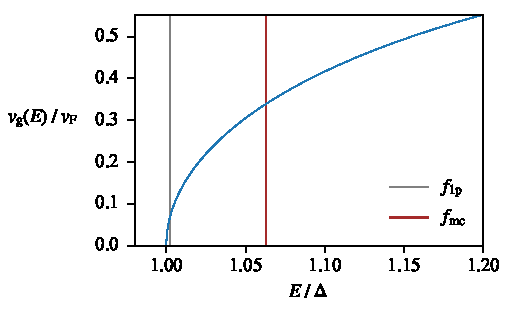
\includegraphics[width=0.9\textwidth]{theory/quasiparticle_group_velocity.pdf}
\caption[The quasiparticle group velocity versus quasiparticle energy.]
{
The quasiparticle group velocity normalized to the Fermi velocity versus quasiparticle energy normalized to the gap energy.
The blue curve is universal.
The vertical lines correspond to the energy of the gap plus one readout photon for the two fiducial readout frequencies, assuming the fiducial value for the gap energy.
We expect the first peaks in the occupancy to occur at these energies.
}
\label{fig:quasiparticle_group_velocity}
\end{figure}

The quasiparticle diffusion coefficient $\qpdiffusion$ is related to the normal-state diffusion coefficient $\normaldiffusion$ by
\begin{equation}
\qpdiffusion
  =
  \frac{\expval{\velocity_\group}}{\velocity_\fermi} \normaldiffusion,
\end{equation}
where $\expval{\velocity_\group}$ is the group velocity averaged over all quasiparticles~\autocite{Ullom1998PRB}.
The rapid variation of the group velocity with energy makes it difficult to estimate the quasiparticle diffusion coefficient without a good estimate of the nonequilibrium occupancy.
Assuming only pair recombination is relevant, a typical diffusion distance is then
$(\qpdiffusion \phonontrapping \qprecombinationtime)^{1/2}$.
This is usually long enough to reduce the problem to two dimensions.
\todo[inline]{Calculate fiducial diffusion length!}

With $\qpdensity(\time, \vb{x})$ the position-dependent density and $\nabla^2$ the Laplacian, both in two dimensions, Equation~\ref{eqn:rate_qpdensity} becomes
\begin{equation}
\pdv{\qpdensity(\time, \vb{x})}{\time}
  =
  \rate_\generation(\time, \vb{x})
  + \qpdiffusion \nabla^2 \qpdensity(\time, \vb{x})
  -\qprecombinationeff \qpdensity(\time, \vb{x})^2
  -\qpsingledecay \qpdensity(\time, \vb{x}).
\label{eqn:rate_qpdensity_diffusion}
\end{equation}
Solutions of similar equations have been attempted~\autocite{Wang2014NatComm,Nsanzineza2014PRL}.
However, when modeling detector response we will assume that the quasiparticle density is homogeneous in some volume $\volume$.
This will allow us to switch freely between quasiparticle density $\qpdensity$ and number $\qpnumber = \volume \qpdensity$.
The readout signal will tend to produce peaks in the occupancy at energies that are greater than the gap by integer multiples of the readout photon energy.
Thus, we expect more rapid diffusion than the thermal average quasiparticle velocity would suggest.
Additionally, since the local recombination time increases rapidly with decreasing density, those quasiparticles that diffuse away from a high-density region may travel much farther than the typical diffusion length in higher-density regions.
In hybrid KIDs, in which quasiparticles are trapped in a high-current region, diffusion tends to equalize the density.
In single-metal KIDs, such as the all-aluminum lumped-element devices discussed here, quasiparticles that diffuse into low-current regions of the capacitors are effectively lost.
